% Parte A: SLAM y generación del mapa.
% Consigna: consignas/PRA_TPFinal_Parte_A.pdf, secciones 3 (evaluación) y 4 (entregables).
% Los números salen de informe/datos/resumen_a.csv y de docs/decisiones/.

\section{Parte A: SLAM y generación del mapa}

El objetivo de esta parte es construir un mapa de ocupación del aula mientras el
robot estima su propia pose, usando solo el LIDAR y la odometría. El mapa que
sale de acá es el que usa la navegación de la parte B.

\paragraph{Datos de entrada.} El scan \code{/scan} de 1080 rayos a 7,3 Hz, la
odometría \code{/odom} a 10 Hz y la terna del LIDAR respecto del robot (0,043 m
adelante, girado 180\textdegree). Seguimos el orden que recomienda la consigna:
primero el café simulado en Gazebo, después el rosbag del TP Parcial y por último
el robot en el aula, donde grabamos dos recorridos completos con rosbag mientras
el SLAM corría en vivo. No hay pose verdadera del robot en el aula ni medidas con
cinta, así que las métricas del aula miden consistencia y no exactitud.

\subsection{Método elegido}

Elegimos FastSLAM sobre grillas de ocupación~\cite{thrun,fastslam,gmapping}: un
filtro de partículas donde cada partícula lleva una hipótesis de trayectoria y
su propio mapa en log-odds. Tres razones. El resultado es directamente una
grilla de ocupación, que es lo que necesita el planificador de la parte B, sin
un paso intermedio de landmarks que en el aula no sabríamos de dónde sacar. Es
online, entonces vemos el mapa crecer mientras manejamos el robot y sabemos en el
momento si una zona quedó sin cubrir. Y reutiliza lo que ya conocíamos del
filtro de partículas de localización: modelo de movimiento, campo de
verosimilitud y resampling. Todo el núcleo es propio, sin librerías de SLAM, y
no depende de ROS, lo que nos permitió repetir cada recorrido offline con otra
configuración sin volver al laboratorio.
\resp{qué método eligieron y por qué}

El filtro se validó en las tres etapas con la misma implementación
(tabla~\ref{tab:etapas}). En simulación y en el bag del Parcial existe una
referencia independiente del SLAM, y ahí el error queda entre 5 y 17 cm.

\begin{table}[t]
  \centering\small
  \caption{Las tres etapas, con 8 partículas y tres semillas. En el aula no hay
    referencia: el número es la mediana de la distancia entre la pose final y la
    inicial de un recorrido que termina donde empezó.}
  \label{tab:etapas}
  \begin{tabular}{@{}lll@{}}
    \toprule
    Etapa & Referencia & Error [cm] \\
    \midrule
    Café en Gazebo & pose del simulador & 12,8--16,8 \\
    Bag del Parcial & localización sobre el & 5,4--5,8 \\
                    & mapa de la cátedra & \\
    Aula & cierre del recorrido & 11,7 \\
    \bottomrule
  \end{tabular}
\end{table}

\subsection{Modificaciones al filtro básico}

El filtro básico mueve cada partícula con la odometría más ruido, la pondera con
el scan y resamplea. Le hicimos cuatro cambios, en orden de impacto.

\textbf{Propuesta con scan matching.} Es el cambio que hizo funcionar al método.
Con la propuesta de odometría, alguna partícula tiene que caer cerca de la pose
real por azar, y como la odometría es mucho menos precisa que el LIDAR eso exige
mucho ruido y muchas partículas. En vez de eso, cada partícula toma la pose que
predice la odometría, prueba una ventana chica alrededor ($\pm 10$ cm y
$\pm 0{,}06$ rad, 1053 poses) y se queda con la que mejor hace coincidir el
scan con su propio mapa, con un prior gaussiano que la mantiene cerca de la
odometría cuando el scan no alcanza para decidir. Es la idea de
GMapping~\cite{gmapping}. En el aula, sin scan matching y con 8 partículas el
recorrido cierra a 31 cm de mediana, una de cada seis corridas termina a más de
50 cm y el contorno del aula sale torcido (figura~\ref{fig:scanmatching}). Con
scan matching cierra a 12 cm. La propuesta de odometría recién iguala ese cierre
con 128 partículas y un ruido de 32 \% del paso, a un costo por actualización
casi tres veces mayor (89 contra 32 ms) y con un mapa menos nítido.

\textbf{Integrar solo cuando el robot se mueve.} Un scan se incorpora cuando el
robot avanzó 8 cm o giró 0,06 rad desde el anterior. Con el robot quieto no se
integra nada, ni siquiera por tiempo.

\textbf{Rayos sin retorno ignorados.} Un rayo que vuelve infinito no marca
espacio libre. En el segundo recorrido del aula son el 27 \% de las lecturas.

\textbf{Resampling selectivo.} Se resamplea solo cuando el número efectivo de
partículas baja de la mitad, con resampling sistemático y pesos en logaritmos.
Resamplear en cada scan copia mapas de más y elimina hipótesis que todavía
servían.
\resp{las modificaciones al filtro vainilla}

\begin{figure*}[t]
  \centering
  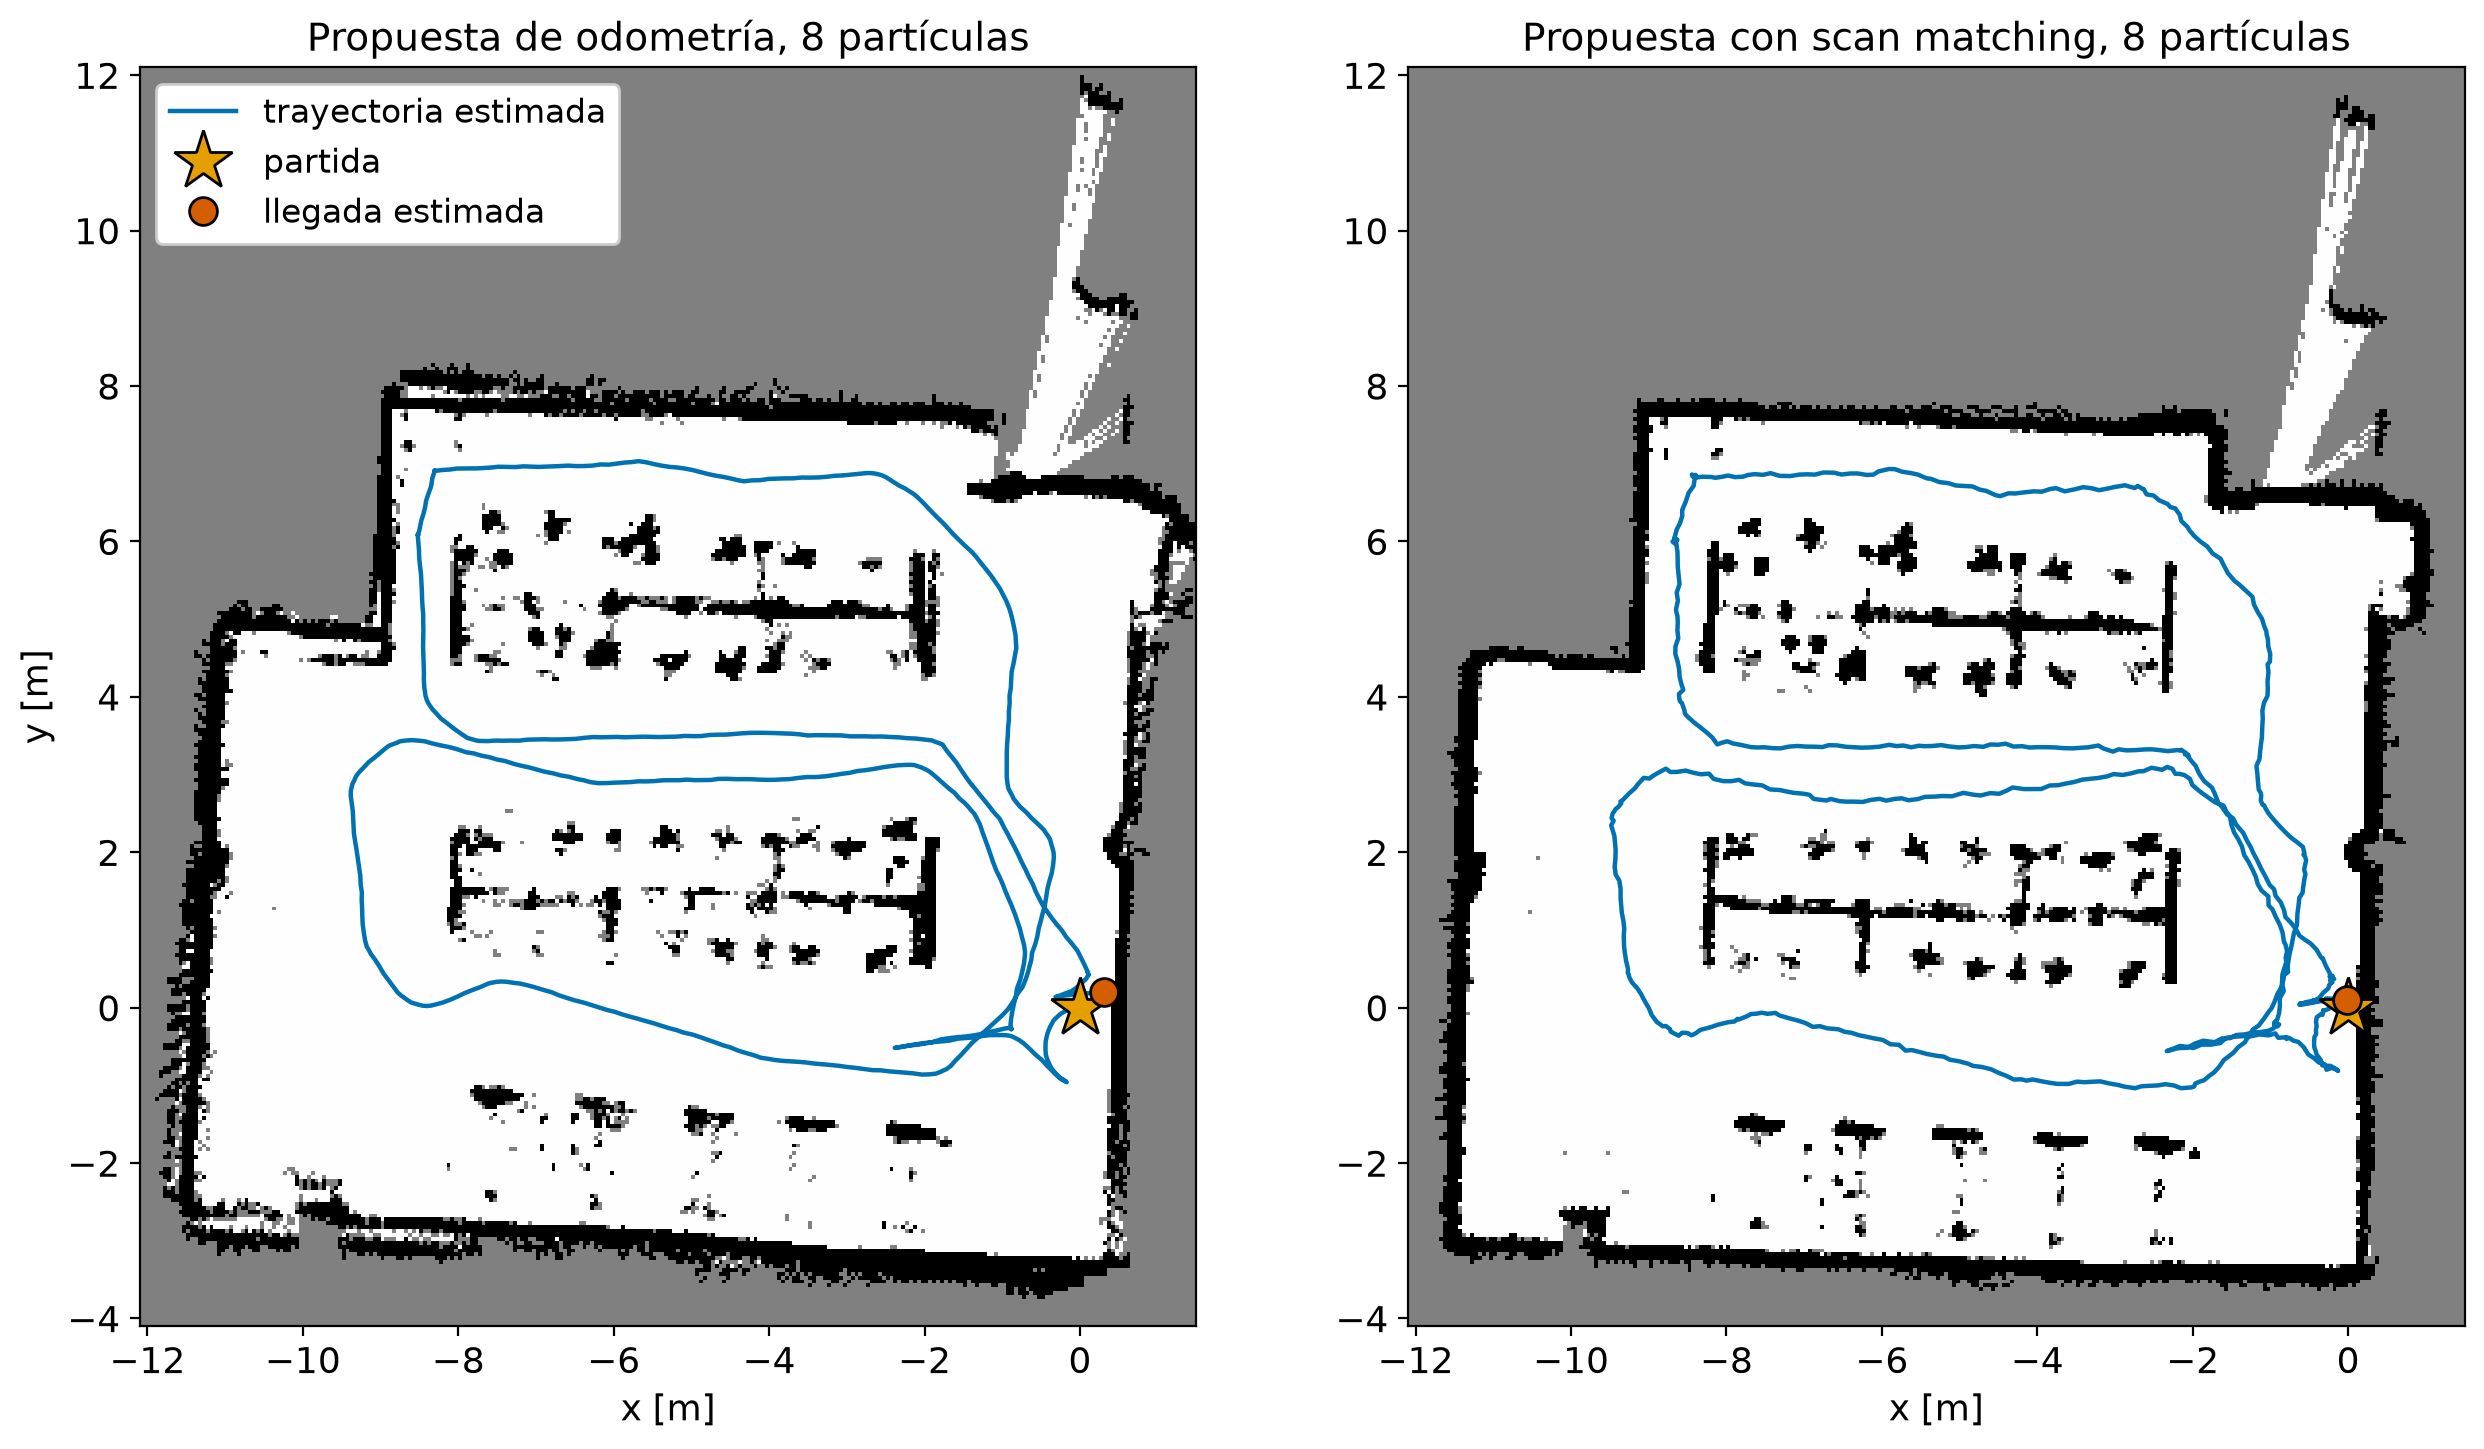
\includegraphics[width=0.92\textwidth]{a_scan_matching}
  \caption{El mismo recorrido del aula y la misma semilla, con la propuesta de
    odometría y con scan matching. Sin scan matching el error de la odometría
    pasa al mapa: las paredes se tuercen y el contorno no cierra.}
  \label{fig:scanmatching}
\end{figure*}

\subsection{Dificultades de desarrollo}

\textbf{El filtro básico no alcanzaba en tiempo real.} En el bag del Parcial la
propuesta de odometría divergía por metros con poco ruido y necesitaba 128
partículas con mucho ruido, a 0,44 s por actualización contra 0,19 s
disponibles. Lo resolvimos con el scan matching, no con más cómputo.

\textbf{Las lecturas sin retorno borraban paredes.} La primera versión trataba
un rayo sin retorno como espacio libre hasta 8 m. Sobre datos reales eso limpia
celdas de pared cada vez que un rayo se pierde en un vidrio o en una superficie
oscura. En el aula, con esa regla la distancia media de los puntos del scan a la
pared del mapa sube de 1,1 a 10,9 cm.

\textbf{La pose se movía con el robot quieto.} El filtro integraba un scan por
segundo aunque no hubiera movimiento, y cada integración sumaba el ruido de la
propuesta. En el segundo recorrido del aula la pose caminó 17 cm en 215 s de
robot estacionado, con la odometría y los scans sin cambiar. Lo detectamos al
comparar el origen del mapa con el lugar físico de partida, y lo corregimos
integrando solo por movimiento.

\textbf{Elegir una métrica que no engañe.} Al principio alineábamos la
trayectoria estimada con la referencia usando solo la primera pose, y un error
de pocos grados al inicio inflaba el error de toda la corrida: la misma corrida
daba entre 8 y 14 cm. Pasamos a un ajuste rígido de la trayectoria completa.

\textbf{El robot real.} El primer mapa del aula salió torcido entre 15
y 20\textdegree{} por girar rápido, hubo que usar \code{base\_footprint} como
terna de la base (con \code{base\_link} el nodo descartaba todos los scans) y
en un reinicio quedaron dos nodos de SLAM publicando el mismo mapa.
\resp{las dificultades de desarrollo}

\subsection{Mapa del aula}

El mapa final (figura~\ref{fig:mapa}) sale del segundo recorrido: 58 m en dos
vueltas alrededor de los dos bloques de mesas, con celdas de 5 cm y 8
partículas. Tiene 109 m\textsuperscript{2} de espacio libre en un aula de unos
$11{,}5 \times 10{,}6$ m.

\textbf{Coherencia con el entorno.} Las paredes salen rectas y sin duplicar, y
se distinguen las mesas y las patas de las sillas. La odometría sola termina a
1,9 m y 21\textdegree{} de la pose final del SLAM, y el SLAM vuelve al punto de
partida con 11,7 cm de mediana sobre 7 semillas. El robot arrancó y terminó
dentro de un recuadro de cinta en el piso, con menos de 10 cm de error al
estacionar, así que ese cierre está en el límite de lo que podemos medir. Las
semillas difieren entre sí 3,3 cm RMS. El mapa del primer recorrido, hecho por
otro camino y arrancando en sentido opuesto, coincide con este en el 95 \% de
las celdas ocupadas a menos de 20 cm. La zona blanca que sale del aula arriba a
la derecha es la puerta de vidrio: el LIDAR ve a través de ella y la pared real
sigue derecha.
\resp{el criterio 3.1}

\textbf{Resolución y detalle.} Con 5 cm se ven los pasillos entre mesas y las
patas de las sillas. Las paredes tienen entre 20 y 25 cm de
grosor en el mapa, más que las reales. No afecta al planificador, porque la cara
interna de la pared está en su lugar, pero es el defecto visible del mapa y lo
analizamos en las preguntas 3 y 6.
\resp{el criterio 3.2}

\textbf{Uso para navegación.} Con la huella del robot inflada 22 cm, el
planificador A* de la parte B encuentra una región transitable de
70,6 m\textsuperscript{2} que llega a todos los pasillos, y entre 40 pares de
puntos al azar planifica en 17 ms de mediana y 90 ms como máximo.
La localización de la parte B sobre este mapa sigue a la trayectoria del SLAM a
3,7 cm con el mismo recorrido y a 4,6 a 4,9 cm con el otro, sin perderse. Dos
límites que conviene conocer: el robot no entró al ala izquierda ni al pasillo
de abajo, que quedaron mapeados desde lejos, y la franja de la puerta figura como
libre.
\resp{el criterio 3.3}

\begin{figure*}[t]
  \centering
  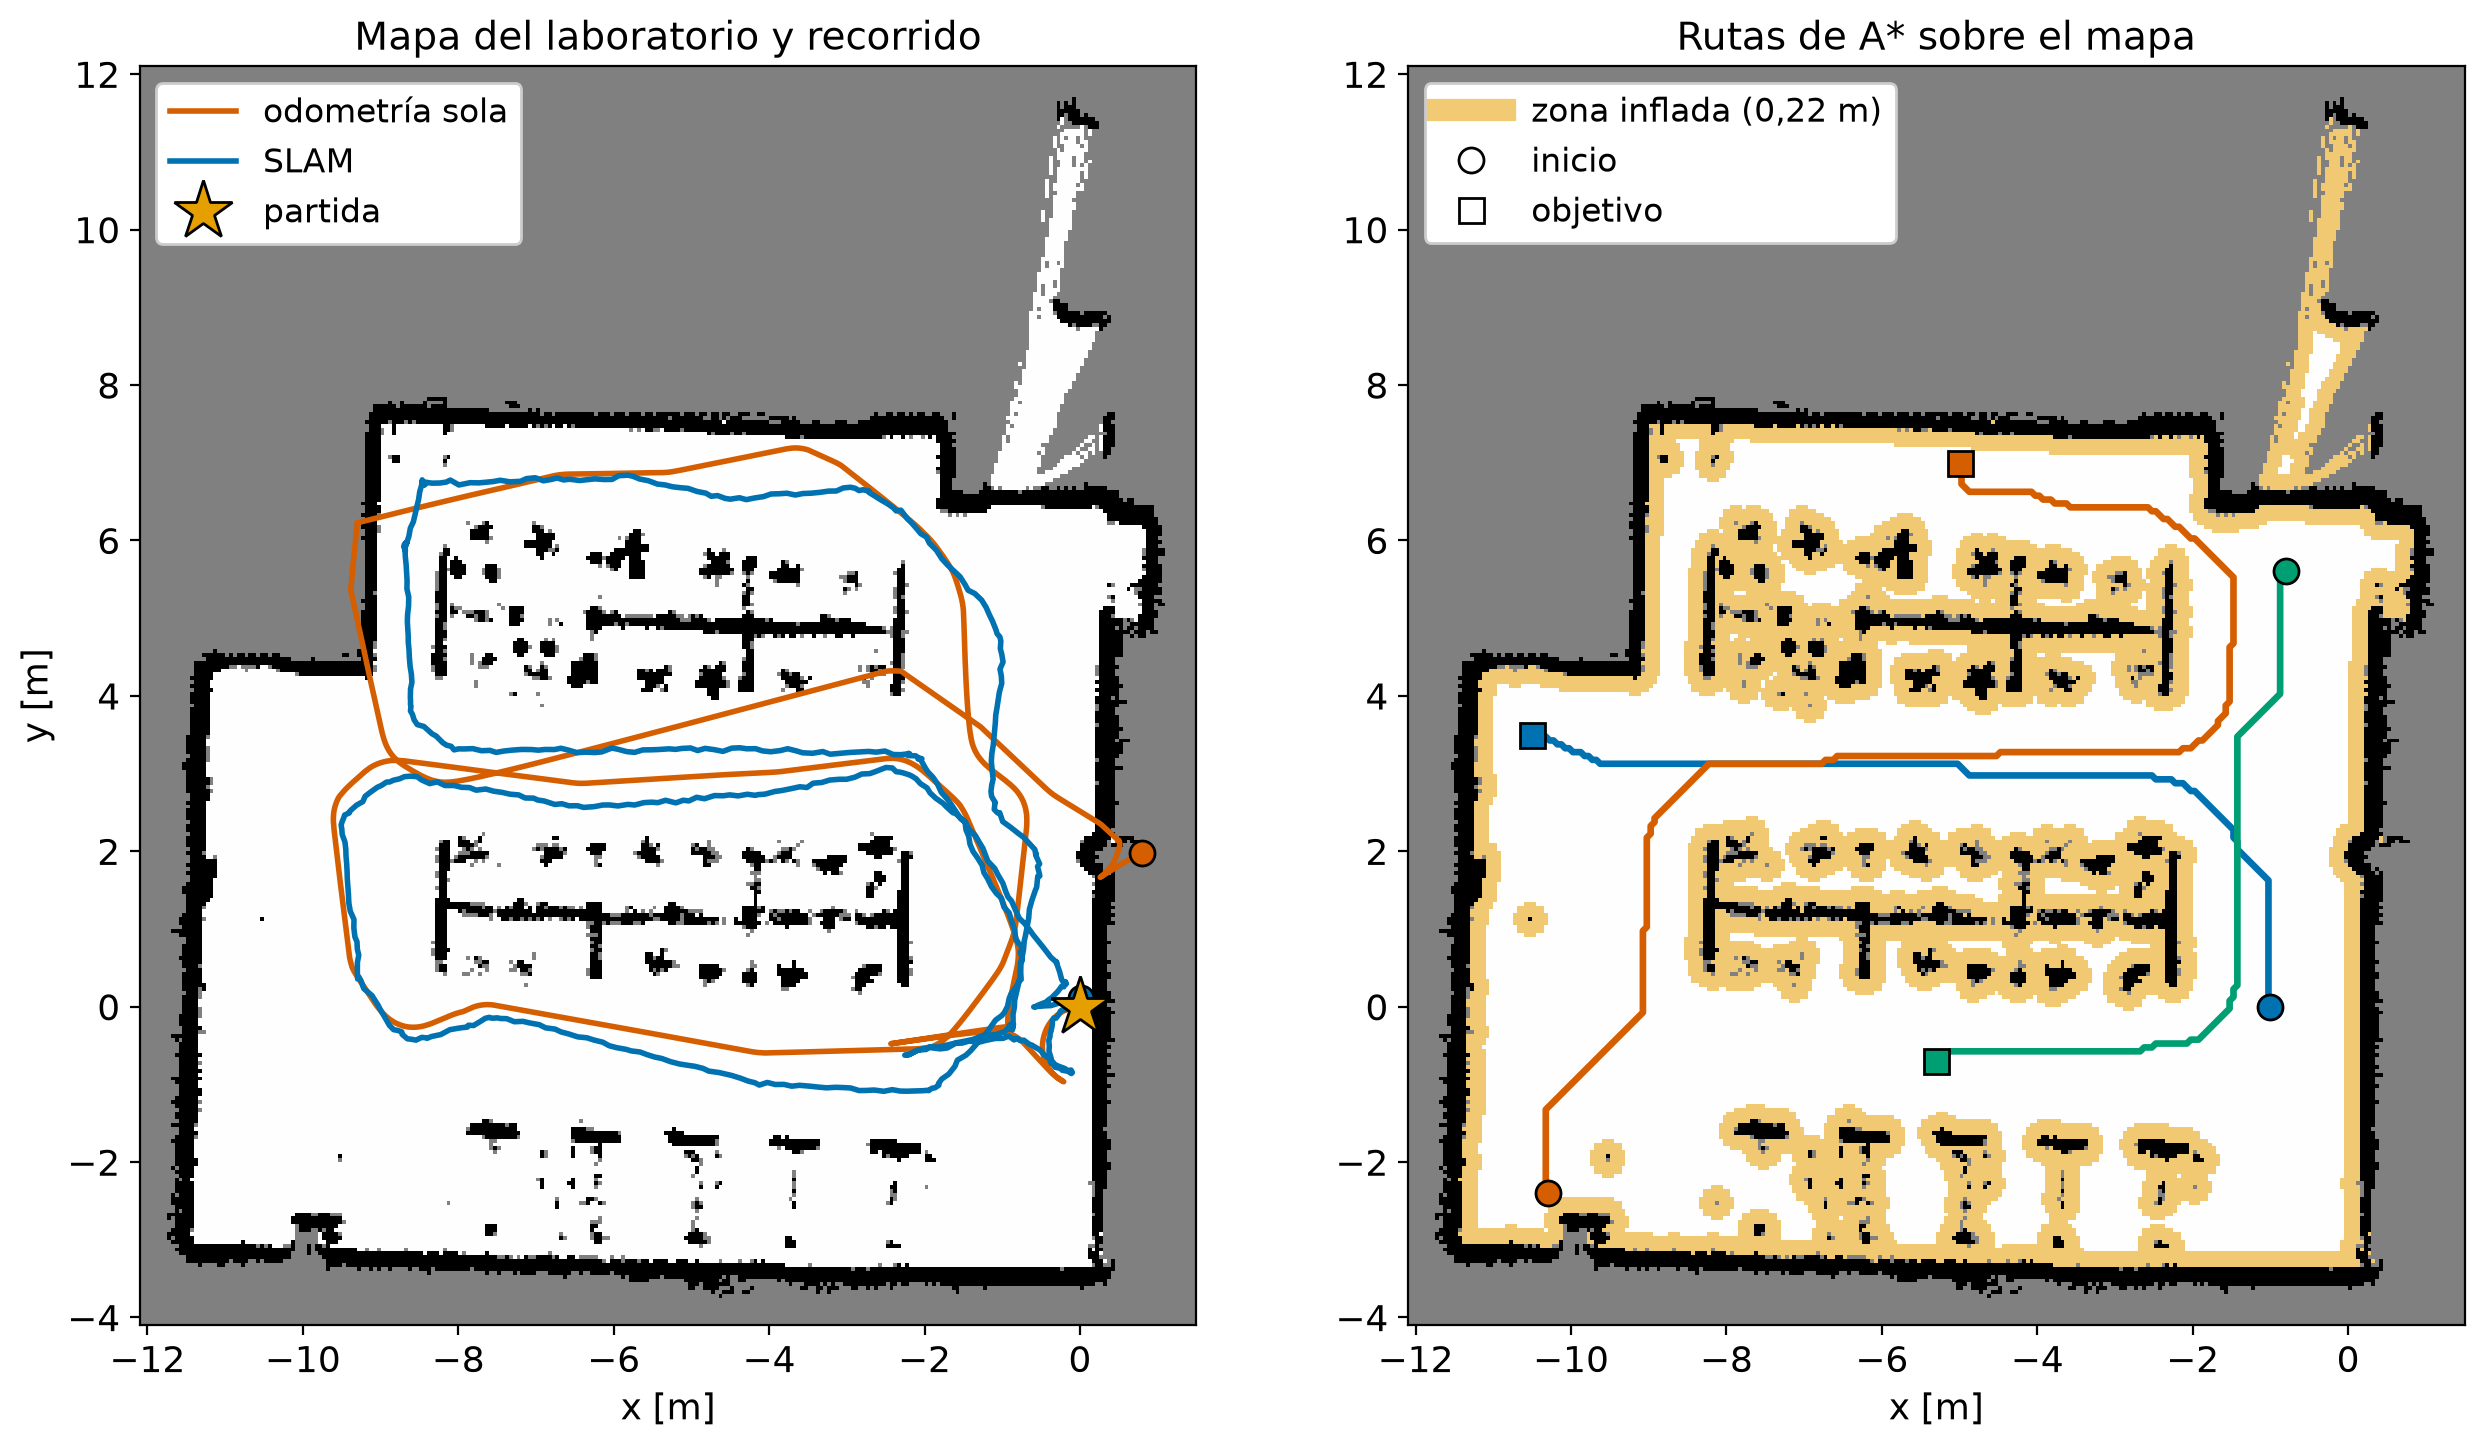
\includegraphics[width=0.92\textwidth]{a_mapa_aula}
  \caption{Izquierda: mapa final del aula con el recorrido estimado por el SLAM y
    el que da la odometría sola (los círculos marcan dónde termina cada uno).
    Derecha: el mismo mapa con la huella del robot inflada y tres rutas de A*.}
  \label{fig:mapa}
\end{figure*}

\subsection{Preguntas}

Para contestar con datos repetimos el segundo recorrido del aula offline
cambiando una sola cosa por vez respecto de la configuración del mapa final, con
6 semillas por caso: 24 configuraciones y 145 corridas. Como no hay pose
verdadera usamos tres medidas de consistencia: el cierre del recorrido, la
dispersión entre semillas y la nitidez, que es la distancia media de los puntos
de cada scan integrado a la celda ocupada más cercana del mapa final
(figura~\ref{fig:sensibilidad}).

\begin{figure*}[t]
  \centering
  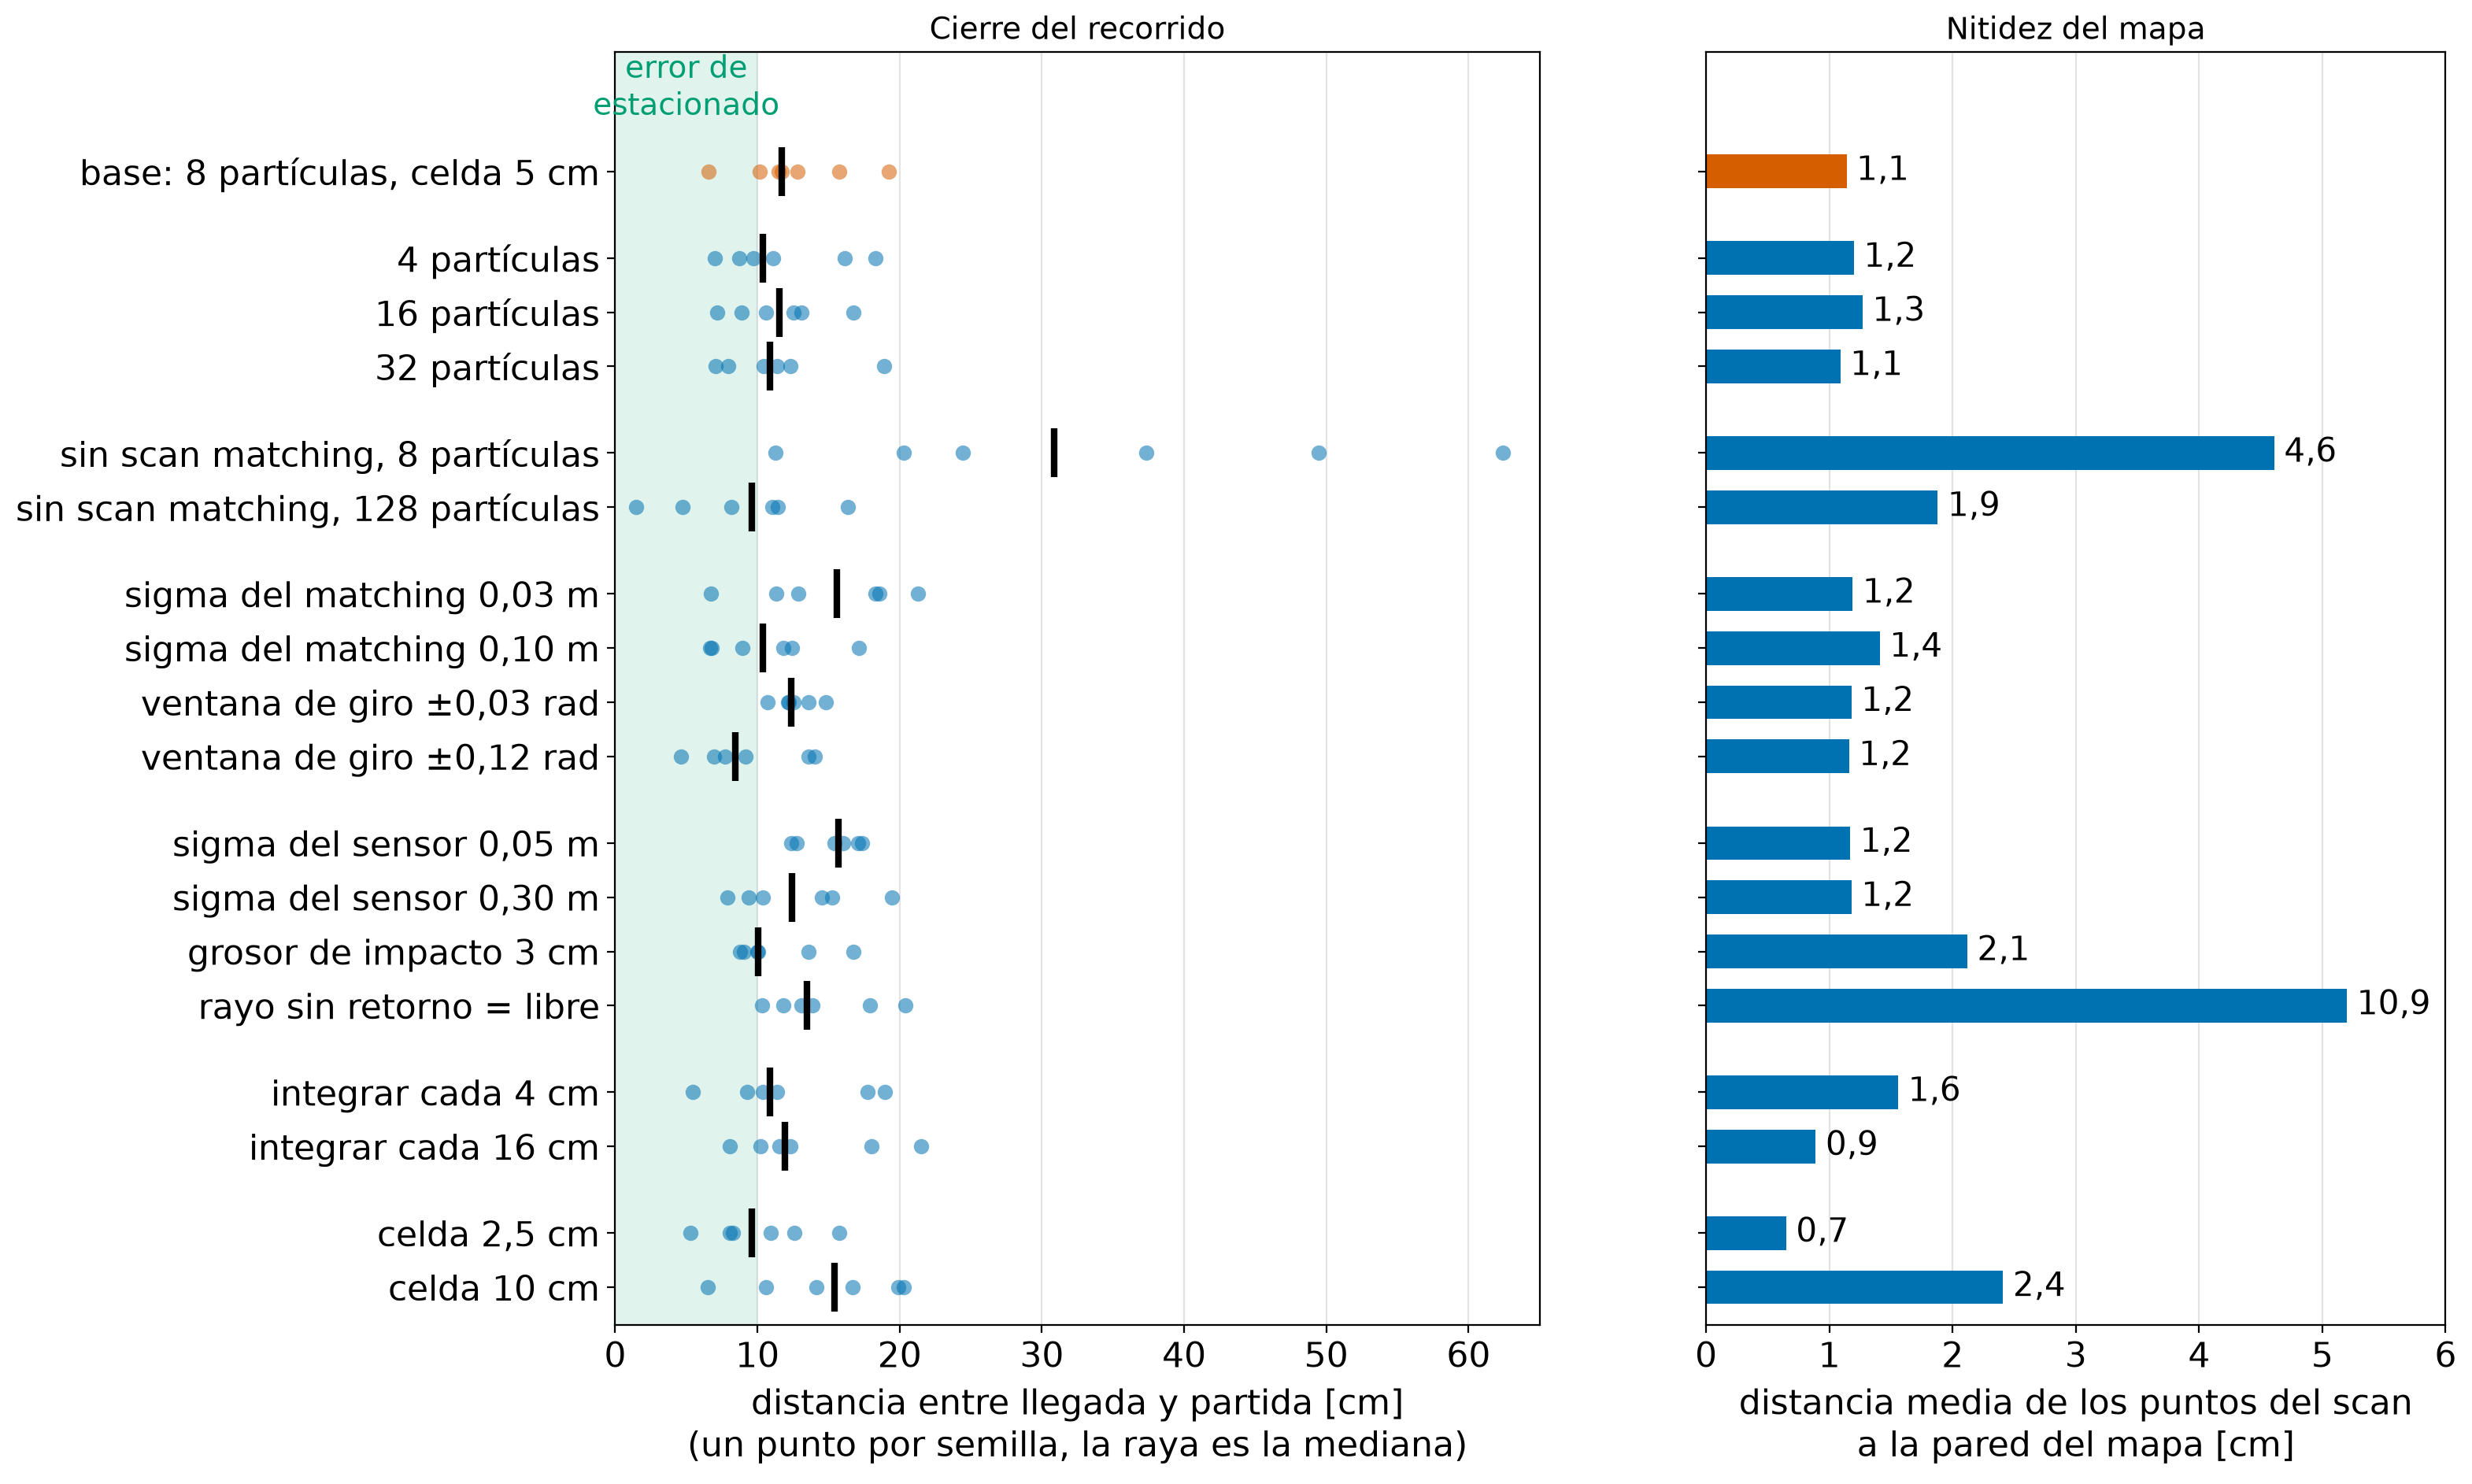
\includegraphics[width=0.95\textwidth]{a_sensibilidad}
  \caption{Efecto de cambiar un parámetro por vez sobre el recorrido del aula.
    La franja verde es el error con que se estacionó el robot: por debajo de
    10 cm el cierre no distingue una configuración de otra.}
  \label{fig:sensibilidad}
\end{figure*}

\subsubsection*{1. \textquestiondown{}Qué tan sensible a hiperparámetros es el método que eligieron? \textquestiondown{}Porqué?}

Con scan matching, poco. De 4 a 32 partículas, con la ventana de giro a la mitad
o al doble y con el sigma del sensor entre 0,05 y 0,30 m, la mediana del cierre
queda entre 8 y 16 cm, dentro de lo que ya varía la configuración base de una
semilla a otra (6 a 19 cm), y ninguna corrida falla. La razón es que el scan
matching ubica cada partícula con el LIDAR, que es preciso, y entonces el ruido
de movimiento y la cantidad de partículas dejan de tener que cubrir el error de
la odometría. Sin scan matching el método es muy sensible: con 8 partículas el
cierre va de 11 a 62 cm según la semilla.

Lo que sí cambia el resultado son los parámetros que definen cómo se escribe el
mapa: la regla de los rayos sin retorno, el tamaño de celda y el grosor con que
se marca cada impacto.

\subsubsection*{2. \textquestiondown{}Tuvieron que hacer un proceso de tueno de parámetros?}

Sí, en dos momentos. Con el bag del Parcial barrimos el ruido de movimiento y la
cantidad de partículas de la propuesta de odometría, y el resultado fue que no
había un punto barato que funcionara. Eso nos llevó a cambiar la propuesta en
vez de seguir ajustando. Después ajustamos sobre el mismo bag el sigma del
sensor (0,15 m) y el grosor de impacto (8 cm), con el error contra la
referencia como criterio.

Para el aula solo agrandamos el mapa a $48 \times 40$ m. El barrido posterior
confirmó que no había nada que ganar: 16 partículas dan el mismo cierre (11,6
contra 11,7 cm) y la misma nitidez que 8, al doble de costo, así que nos
quedamos con 8.

\subsubsection*{3. \textquestiondown{}Al momento de hacer el mapeo, observaron alguna dependencia entre el recorrido que tomaban o la velocidad a la que avanzaban y el resultado del mapa?}

Sí, de las dos. El primer recorrido, de 49 m y por otro camino, es menos
robusto: 2 de 6 semillas terminan a más de 50 cm del punto de partida,
contra ninguna de 7 en el segundo.

Con la velocidad, lo que importa es el giro y no el avance
(figura~\ref{fig:velocidad}). El residuo de un scan se duplica cuando el robot
gira a más de 0,5 rad/s y casi no cambia con la velocidad de avance. El filtro
asigna una sola pose a cada scan, y a 1 rad/s un barrido de 0,137 s abarca
8\textdegree. También probamos descartar scans para simular un robot más rápido:
con uno de cada cuatro el recorrido cierra igual o mejor (7,6 cm), o sea que la
separación entre scans no es el límite. No tenemos un recorrido lento para
comparar de forma controlada: manejamos a 0,4 m/s de mediana y con giros de
hasta 1 rad/s.

\begin{figure}[t]
  \centering
  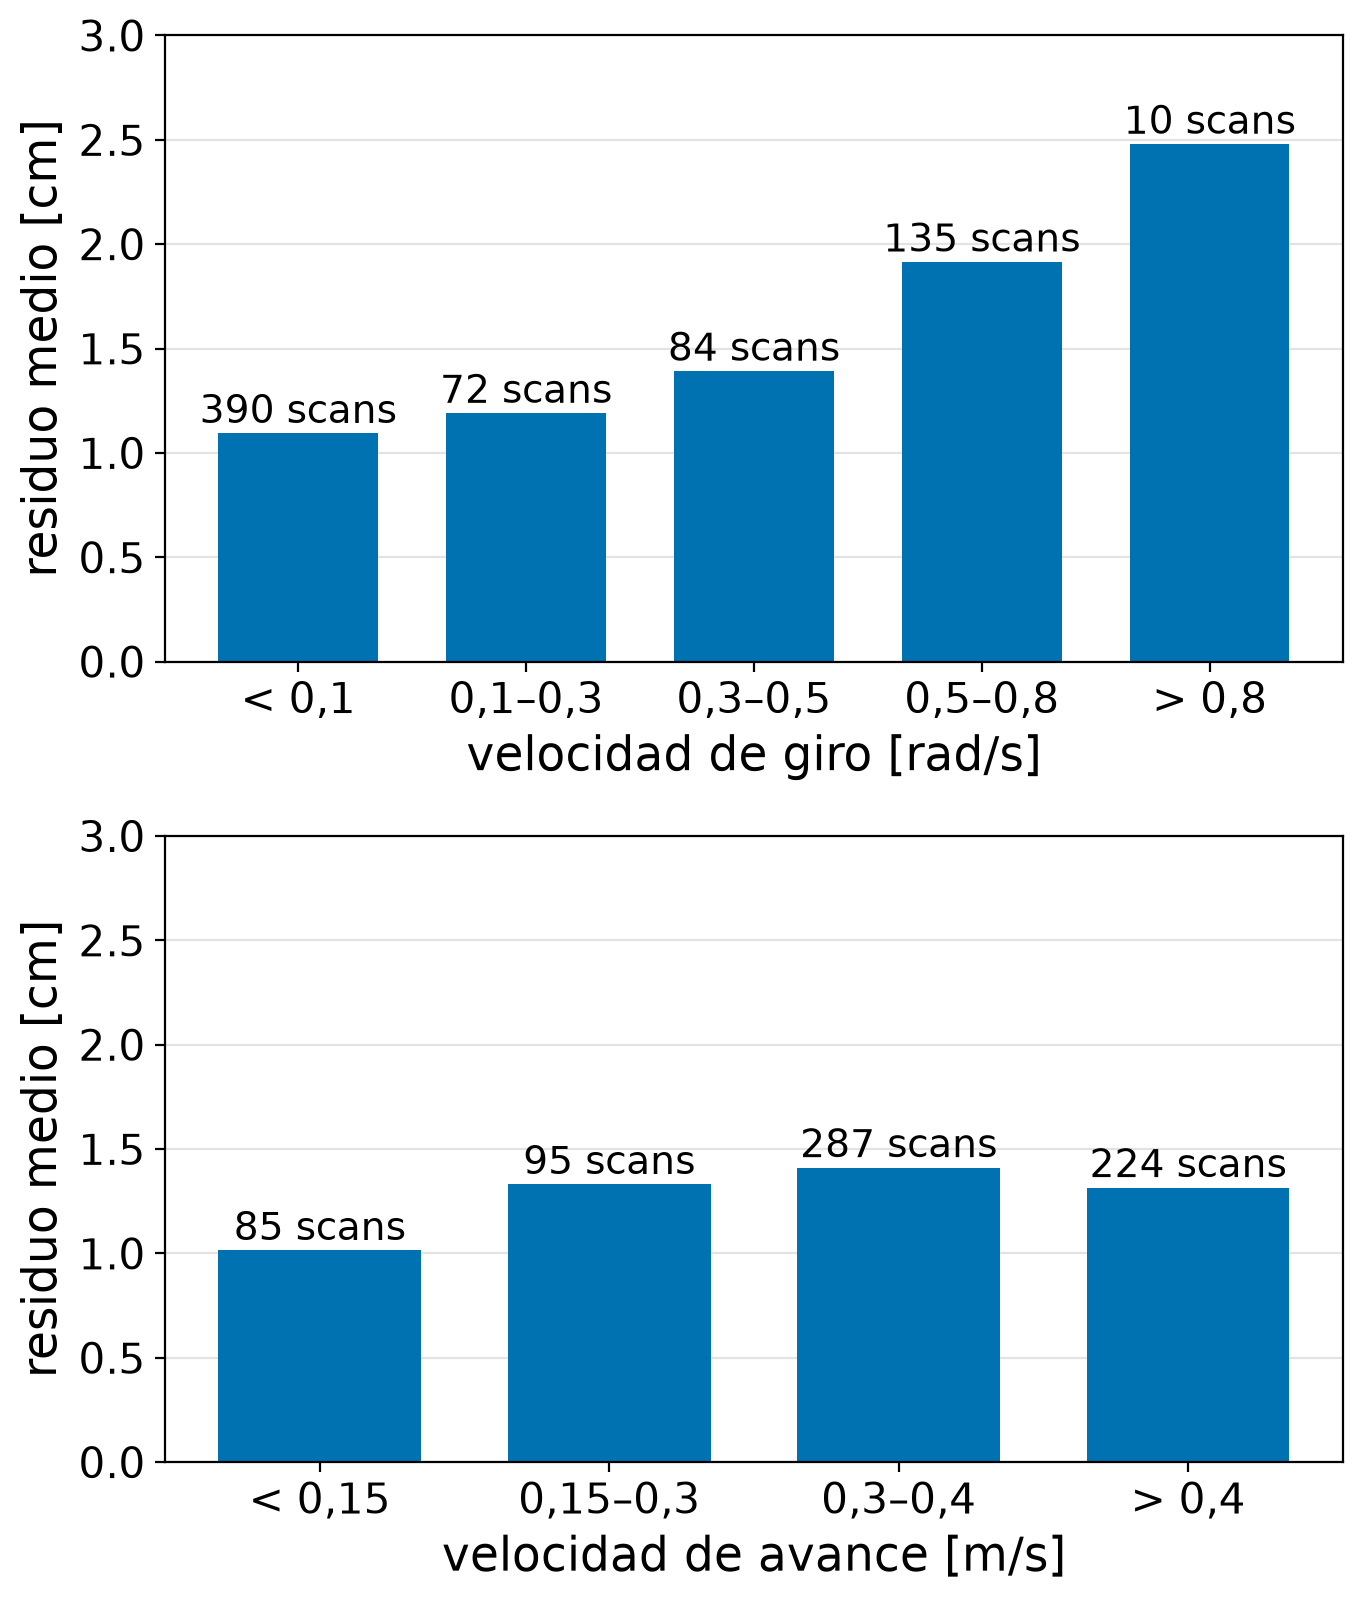
\includegraphics[width=\columnwidth]{a_velocidad}
  \caption{Residuo de cada scan integrado contra el mapa final, según la
    velocidad del robot en ese instante.}
  \label{fig:velocidad}
\end{figure}

\subsubsection*{4. \textquestiondown{}Qué fuentes de error tuvieron mayor impacto en la calidad del mapa: la odometría, el sensor o el propio algoritmo de SLAM? \textquestiondown{}Cómo lo determinaron?}

Lo determinamos quitando o cambiando una pieza por vez sobre el mismo recorrido.

La odometría es la fuente de error más grande en bruto, 1,9 m y 21\textdegree{}
en 58 m, pero es la que mejor se corrige: con scan matching no llega al mapa. El
sensor pesa de dos maneras. Los rayos sin retorno, mal interpretados, son lo que
más daña el mapa de todo lo que probamos (nitidez de 1,1 a 10,9 cm), y la
distorsión del barrido durante los giros es lo que hoy limita la nitidez. El
algoritmo aportó dos errores propios: la pose que se movía con el robot quieto,
ya corregida, y el grosor de las paredes, que depende del grosor de impacto
configurado. Con 3 cm en vez de 8 las paredes bajan de 25 a 15 cm, pero quedan
con huecos y la nitidez empeora de 1,1 a 2,1 cm.

En el mapa final, entonces, pesan más el tratamiento del sensor y las
decisiones del algoritmo que la odometría.

\subsubsection*{5. \textquestiondown{}Qué ocurre si el robot vuelve a pasar por una zona que ya había recorrido? \textquestiondown{}El algoritmo logra corregir errores acumulados? \textquestiondown{}El algoritmo que seleccionaron corrige solo valores locales o también corrige valores lejanos al momento de pasar por una zona nuevamente?}

Cuando el robot vuelve a una zona conocida, el scan matching compara el scan con
las paredes que la partícula ya había mapeado ahí y la pose se vuelve a
enganchar con ellas. Por eso el error no sigue creciendo: después de dos vueltas
y 58 m el recorrido cierra a 12 cm.

La corrección es local. El filtro no recalcula poses pasadas ni reescribe las
celdas que marcó con una pose equivocada. Lo único que puede cambiar el pasado
es el resampling, que al elegir una partícula elige también toda su trayectoria
y su mapa. Con 8 partículas las historias se unifican rápido, así que esa
corrección alcanza pocos pasos hacia atrás. Lo vemos en el primer recorrido: las
dos corridas que terminan a 55 cm no se recuperan al volver al punto de partida.
Un método de grafo sí redistribuiría ese error a lo largo de toda la vuelta.

\subsubsection*{6. \textquestiondown{}Como afecta el tamaño de grillado al mapa resultante? \textquestiondown{}Afecta a la convergencia? \textquestiondown{}Se observan cosas para un grillado que para otro no?}

No afecta a la convergencia: con 2,5, 5 y 10 cm ninguna corrida falla y el
cierre es parecido (tabla~\ref{tab:celda}). Afecta al detalle y al costo. Con
2,5 cm se distingue cada pata de silla y las paredes salen más finas. Con 10 cm
las sillas vecinas se funden en una mancha y se cierran pasos entre ellas
(figura~\ref{fig:celda}), y el scan matching trabaja contra un mapa más grueso.
El costo por actualización crece cerca de cuatro veces al bajar de 5 a 2,5 cm.
Elegimos 5 cm: resuelve los pasillos del aula y deja margen de tiempo.

\begin{table}[t]
  \centering\small
  \caption{Efecto del tamaño de celda, medianas de 6 semillas. El tiempo es por
    actualización en una laptop (Apple M4), corriendo sola.}
  \label{tab:celda}
  \begin{tabular}{@{}lrrr@{}}
    \toprule
    & 2,5 cm & 5 cm & 10 cm \\
    \midrule
    Cierre [cm] & 9,6 & 11,7 & 15,4 \\
    Nitidez [cm] & 0,7 & 1,1 & 2,4 \\
    Grosor de pared [cm] & 17,5 & 25 & 30 \\
    Tiempo [ms] & 117 & 32 & 11 \\
    \bottomrule
  \end{tabular}
\end{table}

\begin{figure*}[t]
  \centering
  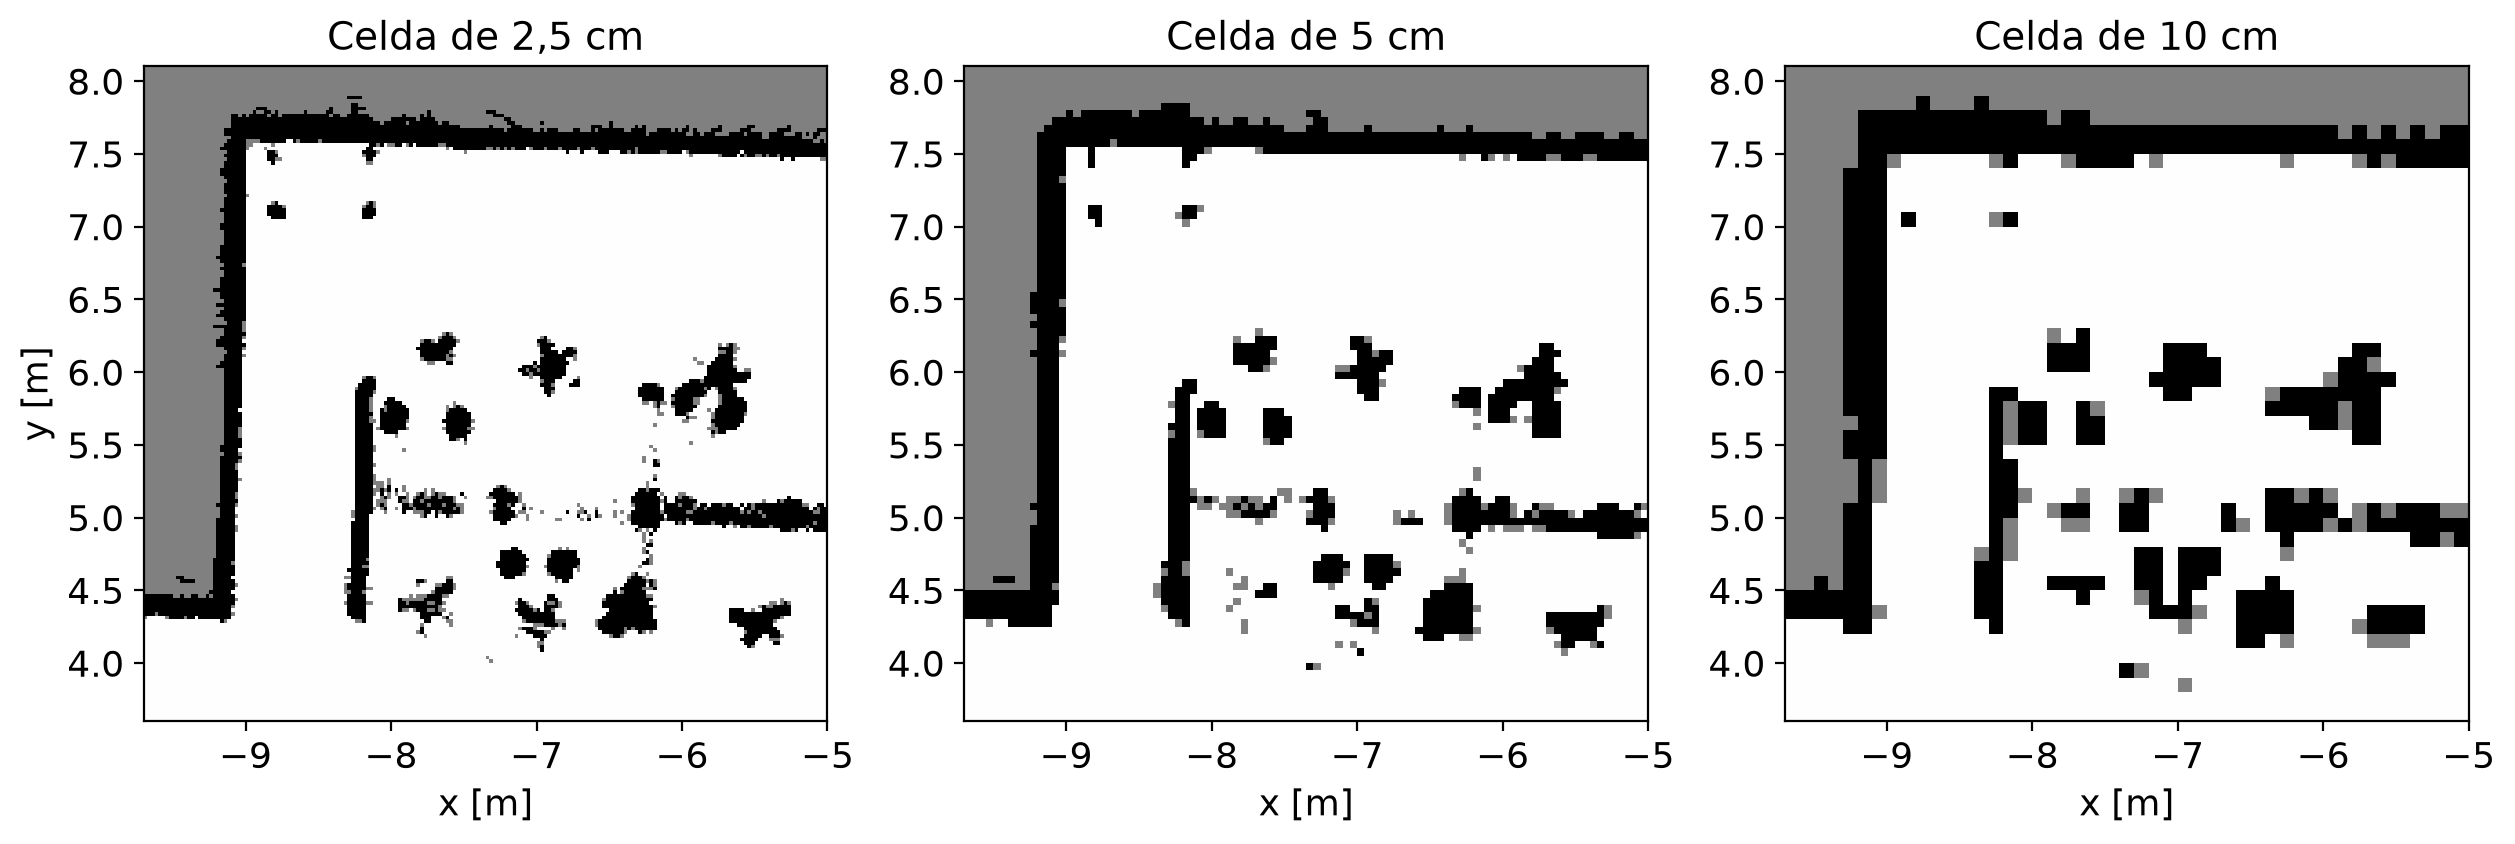
\includegraphics[width=0.95\textwidth]{a_celda}
  \caption{La misma esquina del aula con tres tamaños de celda. Los círculos
    negros son patas de sillas y mesas.}
  \label{fig:celda}
\end{figure*}

\subsubsection*{7. \textquestiondown{}Qué tan exigente a nivel cómputo es el método que eligieron? \textquestiondown{}Funcionaría en una computadora de menor capacidad?}

El costo es proporcional a la cantidad de partículas, porque cada una hace su
propio scan matching (1053 poses por 180 rayos) y actualiza su propia grilla. En
una laptop, una actualización tarda 16, 32, 65 y 136 ms con 4, 8, 16 y 32
partículas. En la PC del laboratorio, con el robot en vivo, tardó entre 80 y
90 ms con 8 partículas, y el LIDAR entrega un scan cada 137 ms: alcanza, sin
mucho margen. La memoria son 8 grillas de $960 \times 800$ celdas.

En una computadora menor funcionaría bajando a 4 partículas, que en el aula dan
el mismo mapa a la mitad del costo, o con celdas de 10 cm. No lo probamos en la
computadora de a bordo del robot.

\subsubsection*{8. \textquestiondown{}El método que eligieron es online u offline? \textquestiondown{}Qué beneficios tiene cada opción?}

Es online: incorpora cada scan cuando llega y publica el mapa mientras el robot
se mueve. Eso nos dejó ver durante el recorrido qué faltaba cubrir y descartar
en el momento un mapa que salía torcido. A cambio tiene que cumplir con el
tiempo entre scans y decide con la información que tiene hasta ese instante.

Un método offline usa el recorrido completo, puede volver sobre las poses
anteriores y corregir un cierre de lazo a lo largo de toda la vuelta, y no tiene
límite de tiempo. No da un mapa mientras se maneja. En la práctica usamos las
dos cosas: el mapa final es una repetición offline del bag con el mismo filtro
online, ya con la corrección del robot quieto.

\subsubsection*{9. \textquestiondown{}Funcionaría su método para otro tipo de robot como por ejemplo un cuadrúpedo? \textquestiondown{}Porqué? \textquestiondown{}En caso que haga falta, que deberían modificar?}

La estructura sirve para cualquier robot que se mueva en un plano con un LIDAR
2D y alguna odometría. El modelo de movimiento ya admite desplazamiento lateral,
y la mala odometría de las patas no sería el problema: el scan matching ya
absorbe un error de 1,9 m en 58 m.

El problema es que el cuerpo de un cuadrúpedo cabecea y se balancea al caminar,
y el plano del LIDAR deja de ser horizontal. Un rayo inclinado pega en el piso o
en otra altura de la pared, y el filtro lo tomaría como un obstáculo. Habría que
agregar una IMU, proyectar cada scan al plano horizontal con la inclinación
medida y descartar los rayos que apuntan al piso.

\subsubsection*{10. \textquestiondown{}Qué tan 'fácil' sería modificar su algoritmo para hacer un mapeo 3D (ignorando la etapa de tueno de parámetros)?}

Difícil. La idea de fondo se conserva, pero cambia cada pieza. La pose pasa de 3
a 6 dimensiones y el sensor tiene que ser 3D. Una grilla densa por partícula
deja de entrar en memoria (el volumen del aula a 5 cm son unas 60 veces más
celdas que el plano) y habría que pasar a una estructura dispersa como un
octree. Y el scan matching por búsqueda exhaustiva no escala: la ventana de 1053
poses en 3 dimensiones se vuelve de millones en 6, así que habría que
reemplazarlo por un método iterativo como ICP. El modelo de movimiento, el
resampling y la organización del código se reutilizan.

\FloatBarrier
